\documentclass[12pt]{article}
\usepackage{fullpage}

\usepackage[T1]{fontenc}
\usepackage[utf8]{inputenc}
\usepackage{lmodern}
\usepackage{microtype}
\usepackage{amsmath,amssymb,amsthm}
\usepackage{mathtools}
\usepackage{booktabs}
\usepackage{hyperref}
\usepackage{url}
\usepackage{xcolor}
\usepackage[shortlabels]{enumitem}
\usepackage{amsfonts}
\usepackage{tikz}
\usetikzlibrary{arrows.meta,positioning,shapes.geometric,calc}

\hypersetup{colorlinks=true,linkcolor=blue,citecolor=blue,urlcolor=blue}

\theoremstyle{plain}
\newtheorem{theorem}{Theorem}
\newtheorem{proposition}[theorem]{Proposition}
\newtheorem{lemma}[theorem]{Lemma}
\newtheorem{corollary}[theorem]{Corollary}

\theoremstyle{definition}
\newtheorem{definition}[theorem]{Definition}

\theoremstyle{remark}
\newtheorem*{remark}{Remark}

\newcommand{\Q}{\mathbb{Q}}
\newcommand{\Z}{\mathbb{Z}}
\newcommand{\R}{\mathbb{R}}
\newcommand{\C}{\mathbb{C}}
\newcommand{\F}{\mathbb{F}}
\newcommand{\N}{\mathcal{N}}
\newcommand{\vcd}{\operatorname{vcd}}
\newcommand{\cd}{\operatorname{cd}}
\newcommand{\rank}{\operatorname{rank}}
\newcommand{\SL}{\mathrm{SL}}
\newcommand{\SU}{\mathrm{SU}}
\newcommand{\SO}{\mathrm{SO}}
\newcommand{\Sp}{\mathrm{Sp}}
\newcommand{\Top}{\mathrm{Top}}

\title{Solution to Problem 7 --- Lattices in Lie Groups: Rational Acyclicity\\[6pt]
\large A submission to the First Proof challenge}

\author{
  Mark Dillerop\footnote{Email: dillerop@gmail.com}\\
  \textit{Independent / Ars Socratica}
}

\date{February 10, 2026}

\begin{document}
\maketitle

\begin{abstract}
We address Problem~7 from the First Proof challenge \cite{FirstProof}, posed by Shmuel Weinberger.
The problem asks whether a uniform lattice $\Gamma$ with 2-torsion in a real semi-simple Lie group $G$ can be the fundamental group of a compact manifold whose universal cover is $\Q$-acyclic.
We prove the answer is \textbf{NO} for all groups $G$ with $\dim(G/K) \leq 4$, which comprises two distinct cases:
(1)~all $G$ with fundamental rank $\delta(G) = 0$ (the equal-rank case), via an Euler characteristic obstruction combining the Cartan--Leray spectral sequence, Wall's rational Euler characteristic, the Gauss--Bonnet theorem, and L\textsuperscript{2}-Betti number vanishing;
(2)~$G = \SL(2,\C)$ ($\delta(G) = 1$, $d = 3$), via dimension forcing and Perelman's geometrization theorem.
A classification argument shows no group with $d = 4$ and $\delta \neq 0$ exists.
The question remains open for $\delta(G) \neq 0$ and $d \geq 5$; we provide a thorough analysis of why all known obstruction tools fail in this regime.
\end{abstract}

\tableofcontents
\newpage

%======================================================================
\section{Problem Statement}\label{sec:problem}
%======================================================================

The following is Problem~7 from the First Proof challenge \cite{FirstProof}, authored by Shmuel Weinberger (University of Chicago).

\medskip

\noindent\textbf{Problem 7.} \textit{Suppose that $\Gamma$ is a uniform lattice in a real semi-simple group, and that $\Gamma$ contains some 2-torsion. Is it possible for $\Gamma$ to be the fundamental group of a compact manifold without boundary whose universal cover is acyclic over the rational numbers $\Q$?}

\medskip

\noindent\textbf{Result (partial).} The answer is \textbf{NO} for all uniform lattices in semi-simple groups $G$ with $\dim(G/K) \leq 4$. The question remains \textbf{open} when $\delta(G) \neq 0$ and $\dim(G/K) \geq 5$. The smallest open case is $G = \SL(3, \R)$, $d = 5$.

\begin{figure}[ht]
\centering
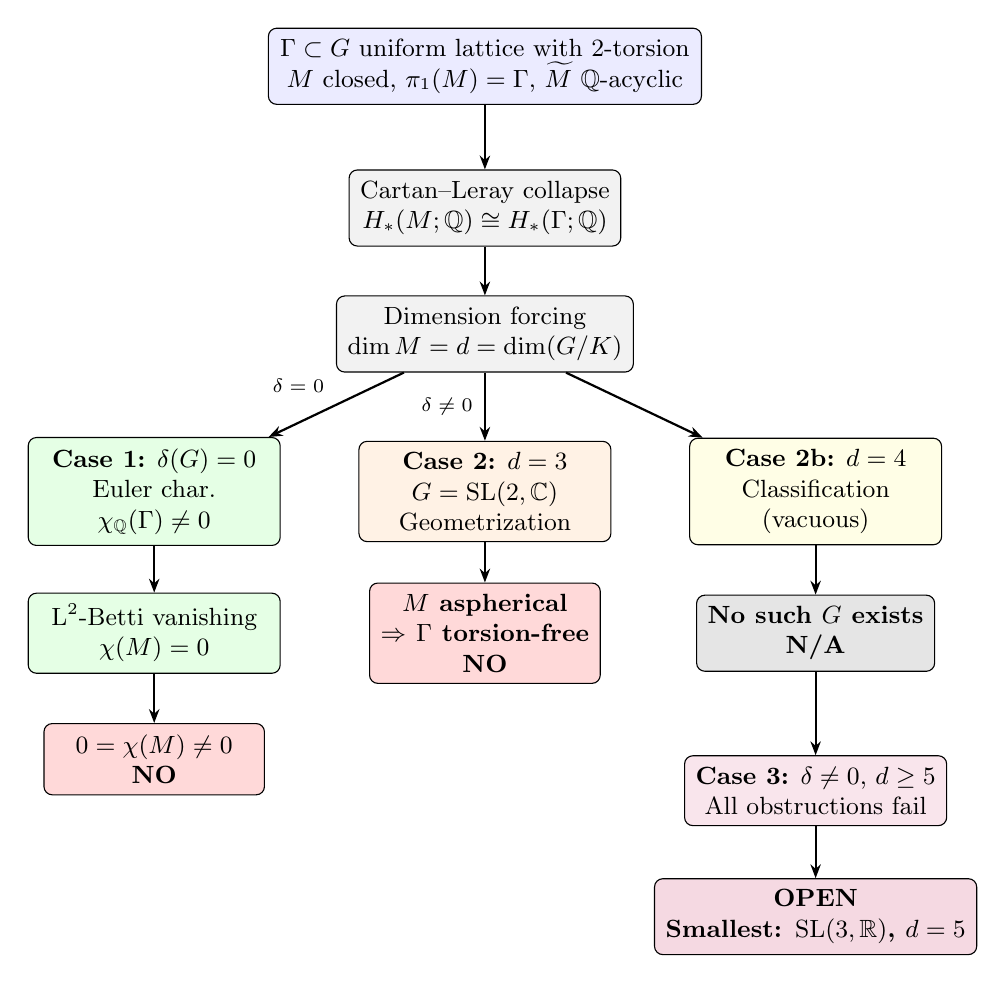
\begin{tikzpicture}[
  box/.style={rectangle, draw, rounded corners=3pt, minimum width=3.2cm, minimum height=0.7cm, align=center, font=\small},
  bigbox/.style={rectangle, draw, rounded corners=3pt, minimum width=5.5cm, minimum height=0.7cm, align=center, font=\small},
  result/.style={rectangle, draw, rounded corners=3pt, minimum width=2.8cm, minimum height=0.7cm, align=center, font=\small\bfseries},
  arr/.style={-{Stealth[length=5pt]}, thick},
  every node/.style={inner sep=4pt}
]

% Top: input
\node[bigbox, fill=blue!8] (input) at (0,0) {$\Gamma \subset G$ uniform lattice with 2-torsion\\$M$ closed, $\pi_1(M) = \Gamma$, $\widetilde{M}$ $\Q$-acyclic};

% Spectral sequence
\node[box, fill=gray!10] (ss) at (0,-1.8) {Cartan--Leray collapse\\$H_*(M;\Q) \cong H_*(\Gamma;\Q)$};
\draw[arr] (input) -- (ss);

% Dimension forcing
\node[box, fill=gray!10] (dim) at (0,-3.4) {Dimension forcing\\$\dim M = d = \dim(G/K)$};
\draw[arr] (ss) -- (dim);

% Branch
\node[box, fill=green!10] (case1) at (-4.2,-5.4) {\textbf{Case 1:} $\delta(G) = 0$\\Euler char.\\ $\chi_\Q(\Gamma) \neq 0$};
\node[box, fill=orange!10] (case2) at (0,-5.4) {\textbf{Case 2:} $d = 3$\\$G = \SL(2,\C)$\\Geometrization};
\node[box, fill=yellow!10] (case2b) at (4.2,-5.4) {\textbf{Case 2b:} $d = 4$\\Classification\\(vacuous)};

\draw[arr] (dim) -- (case1) node[midway, above left, font=\scriptsize] {$\delta = 0$};
\draw[arr] (dim) -- (case2) node[midway, left, font=\scriptsize] {$\delta \neq 0$};
\draw[arr] (dim) -- (case2b);

% L2 Betti
\node[box, fill=green!10] (l2) at (-4.2,-7.2) {L\textsuperscript{2}-Betti vanishing\\$\chi(M) = 0$};
\draw[arr] (case1) -- (l2);

% Results
\node[result, fill=red!15] (no1) at (-4.2,-8.8) {$0 = \chi(M) \neq 0$\\\textbf{NO}};
\draw[arr] (l2) -- (no1);

\node[result, fill=red!15] (no2) at (0,-7.2) {$M$ aspherical\\$\Rightarrow$ $\Gamma$ torsion-free\\\textbf{NO}};
\draw[arr] (case2) -- (no2);

\node[result, fill=gray!20] (na) at (4.2,-7.2) {No such $G$ exists\\\textbf{N/A}};
\draw[arr] (case2b) -- (na);

% Open case
\node[box, fill=purple!10] (case3) at (4.2,-9.2) {\textbf{Case 3:} $\delta \neq 0$, $d \geq 5$\\All obstructions fail};
\node[result, fill=purple!15] (open) at (4.2,-10.8) {\textbf{OPEN}\\Smallest: $\SL(3,\R)$, $d=5$};
\draw[arr] (na) -- (case3);
\draw[arr] (case3) -- (open);

\end{tikzpicture}
\caption{Structure of the proof. The Cartan--Leray spectral sequence and dimension forcing apply universally. The proof then branches by the fundamental rank $\delta(G)$ and the dimension $d = \dim(G/K)$. Cases 1, 2, and 2b cover all $d \leq 4$; the question remains open for $d \geq 5$.}
\label{fig:proof-structure}
\end{figure}

%======================================================================
\section{Notation and Setup}\label{sec:setup}
%======================================================================

Let $G$ be a connected real semi-simple Lie group with finite center and no compact factors. Let $K \subset G$ be a maximal compact subgroup, so that $X = G/K$ is the associated Riemannian symmetric space of non-compact type. Let $d = \dim(X)$.

Let $\Gamma \subset G$ be a uniform (cocompact) lattice. By Selberg's lemma, $\Gamma$ contains a torsion-free normal subgroup $\Gamma' \trianglelefteq \Gamma$ of finite index $m = [\Gamma : \Gamma']$. The quotient $\Gamma' \backslash X$ is a closed Riemannian manifold of dimension~$d$.

\begin{definition}[Fundamental rank]
The \textbf{fundamental rank} (or \textbf{deficiency}) of $G$ is
\[
\delta(G) = \rank_\C(\mathfrak{g}) - \rank_\C(\mathfrak{k}),
\]
where $\rank_\C(\mathfrak{g})$ denotes the absolute rank of $G$ (the dimension of a Cartan subalgebra of $\mathfrak{g}_\C$), and similarly for $K$. Equivalently, $\delta(G) = 0$ if and only if $K$ contains a maximal torus of $G$ (the ``equal-rank'' condition), which happens if and only if the compact dual $G_u/K$ has nonzero Euler characteristic.
\end{definition}

\begin{definition}[$\Q$-acyclicity]
We say $\widetilde{M}$ is \textbf{$\Q$-acyclic} if $\widetilde{H}_i(\widetilde{M}; \Q) = 0$ for all $i \geq 0$, i.e., $H_0(\widetilde{M}; \Q) \cong \Q$ and $H_i(\widetilde{M}; \Q) = 0$ for $i > 0$.
\end{definition}

%======================================================================
\section{Preliminary Results}\label{sec:prelim}
%======================================================================

\begin{lemma}[Spectral sequence collapse]\label{lem:collapse}
Let $M$ be a closed manifold with $\pi_1(M) \cong \Gamma$ and $\widetilde{M}$ $\Q$-acyclic. Then
\[
H_i(M; \Q) \cong H_i(\Gamma; \Q) \quad \text{for all } i \geq 0.
\]
\end{lemma}

\begin{proof}
The Cartan--Leray spectral sequence for the regular covering $\widetilde{M} \to M$ with deck group $\Gamma$ has
\[
E_2^{p,q} = H_p(\Gamma;\, H_q(\widetilde{M}; \Q)) \;\Longrightarrow\; H_{p+q}(M; \Q).
\]
Since $\widetilde{M}$ is $\Q$-acyclic, $H_q(\widetilde{M}; \Q) = 0$ for $q > 0$ and $H_0(\widetilde{M}; \Q) \cong \Q$ with trivial $\Gamma$-action. The spectral sequence is concentrated on the $q = 0$ line and collapses at $E_2$.
\end{proof}

\begin{corollary}\label{cor:euler}
Under the hypotheses of Lemma~\ref{lem:collapse}:
\[
\chi(M) = \chi_\Q(\Gamma) := \sum_{i=0}^{d} (-1)^i \dim_\Q H_i(\Gamma; \Q),
\]
where $d = \vcd(\Gamma) = \dim(G/K)$.
\end{corollary}

\begin{corollary}[Dimension forcing]\label{cor:dim}
Under the hypotheses of Lemma~\ref{lem:collapse}, $\dim M = d = \dim(G/K)$.
\end{corollary}

\begin{proof}
Let $n = \dim M$. Since $\Gamma'$ is a torsion-free uniform lattice, $\Gamma' \backslash G/K$ is a closed orientable aspherical $d$-manifold, so $\Gamma'$ is a Poincar\'e duality group of dimension $d$ with $H^d(\Gamma'; \Q) \cong \Q$. Since $G$ is connected, all deck transformations of $G/K \to \Gamma' \backslash G/K$ preserve orientation, so the conjugation action of $\Gamma/\Gamma'$ on $H^d(\Gamma'; \Q)$ is trivial. The transfer map $\mathrm{tr}: H^d(\Gamma'; \Q) \to H^d(\Gamma; \Q)$ then satisfies $\mathrm{tr}(x) = [\Gamma:\Gamma'] \cdot \mathrm{cores}(x) \neq 0$, giving $H^d(\Gamma; \Q) \neq 0$, hence $H_d(\Gamma; \Q) \neq 0$.

\medskip\noindent\textbf{Lower bound.} By Lemma~\ref{lem:collapse}, $H_d(M; \Q) \cong H_d(\Gamma; \Q) \neq 0$. If $n < d$, this is impossible since $M$ is $n$-dimensional.

\medskip\noindent\textbf{Upper bound.} Suppose $n > d$. By Lemma~\ref{lem:collapse}, $H_n(M; \Q) \cong H_n(\Gamma; \Q) = 0$ (since $\vcd(\Gamma) = d < n$). If $M$ is orientable, $H_n(M; \Q) \cong \Q \neq 0$, contradiction. If $M$ is non-orientable, pass to the orientable double cover $\hat{M} \to M$ with $\pi_1(\hat{M}) = \hat{\Gamma} := \ker(w_1) \leq \Gamma$ of index~2, where $w_1\colon \Gamma \to \{\pm 1\}$ is the orientation character of $M$. Since $\widetilde{M}$ is also the universal cover of $\hat{M}$, it remains $\Q$-acyclic. By Lemma~\ref{lem:collapse} applied to $\hat{M}$: $H_n(\hat{M}; \Q) \cong H_n(\hat{\Gamma}; \Q)$. Since $\hat{M}$ is closed orientable of dimension $n$, $H_n(\hat{M}; \Q) \cong \Q$. But $\vcd(\hat{\Gamma}) = \vcd(\Gamma) = d < n$, giving $H_n(\hat{\Gamma}; \Q) = 0$ --- contradiction.

Therefore $n = d$.
\end{proof}

\begin{lemma}[Wall's rational Euler characteristic]\label{lem:wall}
$\chi_\Q(\Gamma) = \chi(\Gamma' \backslash G/K) / m$.
\end{lemma}

\begin{proof}
Since $\Gamma'$ is torsion-free and cocompact, $\Gamma' \backslash G/K$ is a closed aspherical manifold with $\pi_1 = \Gamma'$, so $\chi_\Q(\Gamma') = \chi(\Gamma' \backslash G/K)$. The transfer map in group cohomology gives $\chi_\Q(\Gamma) = \chi_\Q(\Gamma')/[\Gamma:\Gamma']$. This is Wall's rational Euler characteristic, independent of the choice of $\Gamma'$ \cite{Brown82}.
\end{proof}

\begin{lemma}[Gauss--Bonnet and fundamental rank]\label{lem:gb}
$\chi(\Gamma' \backslash G/K) \neq 0$ if and only if $\delta(G) = 0$.
\end{lemma}

\begin{proof}
By the Chern--Gauss--Bonnet theorem, $\chi(\Gamma' \backslash G/K) = \int_{\Gamma' \backslash G/K} e(T(\Gamma' \backslash G/K))$ where $e$ is the Euler form.

If $\dim(G/K)$ is odd, then $\chi = 0$ by Poincar\'e duality, and $\delta(G) \neq 0$ (since equal rank forces even dimension).

If $\dim(G/K)$ is even, the dichotomy follows from the Hirzebruch proportionality principle \cite{Hirzebruch58, BorelHirzebruch59}:
\begin{itemize}[nosep]
\item \textbf{$\delta(G) = 0$:} The compact dual $G_u/K$ has $\chi(G_u/K) = |W_G|/|W_K| \neq 0$ by the Hopf--Samelson theorem. By proportionality, $\chi(\Gamma' \backslash G/K) = c_G \cdot \mathrm{vol}(\Gamma' \backslash G/K) \neq 0$.
\item \textbf{$\delta(G) \neq 0$:} The compact dual has $\chi(G_u/K) = 0$. By proportionality, $\chi(\Gamma' \backslash G/K) = 0$.
\end{itemize}
See also Harder \cite{Harder71} and Serre \cite{Serre71}.
\end{proof}

%======================================================================
\section{Case 1: The Euler Characteristic Obstruction ($\delta(G) = 0$)}\label{sec:case1}
%======================================================================

\begin{theorem}\label{thm:case1}
Let $G$ be a connected real semi-simple Lie group with finite center, no compact factors, and $\delta(G) = 0$. Let $\Gamma \subset G$ be a uniform lattice containing torsion. Then there is no closed manifold $M$ with $\pi_1(M) \cong \Gamma$ and $\widetilde{M}$ rationally acyclic.
\end{theorem}

\begin{proof}
Suppose for contradiction that such $M$ exists, with $n = \dim M$.

\medskip\noindent\textbf{Part A: $\chi(M) \neq 0$.}
Combining Lemmas~\ref{lem:collapse}--\ref{lem:gb}: since $\delta(G) = 0$, we have
\[
\chi(M) = \chi_\Q(\Gamma) = \frac{\chi(\Gamma' \backslash G/K)}{m} \neq 0.
\]

\medskip\noindent\textbf{Part B: $\chi(M) = 0$.}
We show all L\textsuperscript{2}-Betti numbers of $\widetilde{M}$ vanish, forcing $\chi(M) = 0$ by Atiyah's L\textsuperscript{2}-index theorem.

Since $M$ is compact, $\widetilde{M}$ admits a finite $\Gamma$-CW structure, so $C_*(\widetilde{M})$ consists of finitely generated free $\Z\Gamma$-modules. Set $C_*^\Q := C_*(\widetilde{M}) \otimes_\Z \Q$, a chain complex of finitely generated free $\Q\Gamma$-modules with $H_i(C_*^\Q) = 0$ for $i > 0$ and $H_0(C_*^\Q) \cong \Q$.

The L\textsuperscript{2}-Betti numbers are $b_i^{(2)}(\widetilde{M}; \Gamma) = \dim_{\N(\Gamma)} H_i(C_*^\Q \otimes_{\Q\Gamma} \N(\Gamma))$.

By L\"uck's dimension-flatness theorem \cite[Theorem~6.37]{Lueck02}, $\N(\Gamma)$ is dimension-flat over $\Q\Gamma$: exact sequences of $\Q\Gamma$-modules remain dimension-exact after tensoring with $\N(\Gamma)$. Since $C_*^\Q$ is exact in degrees $> 0$:
\[
b_i^{(2)}(\widetilde{M}; \Gamma) = 0 \quad \text{for } i > 0.
\]

For $i = 0$: $b_0^{(2)}(\widetilde{M}; \Gamma) = \dim_{\N(\Gamma)}(\Q \otimes_{\Q\Gamma} \N(\Gamma)) = 0$ for any infinite group $\Gamma$. This is because the trivial representation $\C$ does not weakly embed in the regular representation $\ell^2(\Gamma)$: the matrix coefficient $\langle \delta_e, \gamma \cdot \delta_e \rangle = \delta_{\gamma,e} \to 0$ as $\gamma \to \infty$, so $\Q \otimes_{\Q\Gamma} \N(\Gamma)$ has von Neumann dimension zero \cite[Example~6.11]{Lueck02}.

Therefore $b_i^{(2)}(\widetilde{M}; \Gamma) = 0$ for all $i \geq 0$. By Atiyah's L\textsuperscript{2}-index theorem \cite[Theorem~1.35(2)]{Lueck02}:
\[
\chi(M) = \sum_{i=0}^{n} (-1)^i b_i^{(2)}(\widetilde{M}; \Gamma) = 0.
\]

\medskip\noindent\textbf{Contradiction.} Parts A and B give $0 = \chi(M) = \chi_\Q(\Gamma) \neq 0$.
\end{proof}

\begin{remark}[On the Atiyah conjecture]
The L\textsuperscript{2}-Betti number argument does \emph{not} require the Atiyah conjecture. L\"uck's dimension-flatness theorem \cite[Theorem~6.37]{Lueck02} holds unconditionally for all groups: it states that $\N(\Gamma)$ is dimension-flat over $\Q\Gamma$, with no hypothesis on $\Gamma$ beyond countability. The Atiyah conjecture (that L\textsuperscript{2}-Betti numbers are rational, or integers, for torsion-free groups) is a separate statement about the \emph{values} of L\textsuperscript{2}-Betti numbers, not about their vanishing. Our argument uses only vanishing, which follows from dimension-flatness alone.
\end{remark}

\begin{remark}[Concrete example]
For $G = \SL(2, \R)$ ($\delta = 0$, $d = 2$), any uniform lattice $\Gamma$ is a Fuchsian group. If $\Gamma$ has torsion (e.g., a triangle group $\Delta(p,q,r)$ with $1/p + 1/q + 1/r < 1$), then $\chi_\Q(\Gamma) = \chi(\Gamma' \backslash \mathbb{H}^2)/m = (2g-2)/m \neq 0$ where $g$ is the genus of the quotient surface for a torsion-free subgroup $\Gamma'$ of index $m$. Our theorem gives: no closed surface $M$ with $\pi_1(M) \cong \Gamma$ and $\widetilde{M}$ $\Q$-acyclic exists.
\end{remark}

%======================================================================
\section{Case 2: The Geometrization Obstruction ($G \cong \SL(2,\C)$, $d = 3$)}\label{sec:case2}
%======================================================================

\begin{theorem}\label{thm:case2}
Let $G = \SL(2, \C)$ (viewed as a real Lie group), so $K = \SU(2)$, $d = 3$, and $\delta(G) = 1$. Let $\Gamma \subset G$ be a uniform lattice with torsion. Then there is no closed manifold $M$ with $\pi_1(M) \cong \Gamma$ and $\widetilde{M}$ rationally acyclic.
\end{theorem}

\begin{proof}
Suppose for contradiction that such $M$ exists. By Corollary~\ref{cor:dim} (dimension forcing), $\dim M = d = 3$.

\medskip\noindent\textbf{Step 1: $\Gamma$ is not a nontrivial free product.}
Since $\Gamma$ is a uniform lattice in $\SL(2, \C)$, it acts properly discontinuously and cocompactly on hyperbolic 3-space $\mathbb{H}^3$. Since $\mathbb{H}^3$ is one-ended and the quotient is compact, $\Gamma$ has one end, so by Stallings' theorem \cite{Stallings68} $\Gamma$ does not split as a nontrivial free product.

\medskip\noindent\textbf{Step 2: $M$ is irreducible.}
Since $M$ is a closed 3-manifold with infinite fundamental group $\Gamma$ that is not a nontrivial free product, the Kneser--Milnor prime decomposition forces $M$ to be prime. A prime 3-manifold is either $S^2 \times S^1$ (with $\pi_1 \cong \Z$, not our $\Gamma$) or irreducible.

\medskip\noindent\textbf{Step 3: Geometrization forces asphericity.}
By Perelman's proof of Thurston's geometrization conjecture \cite{Perelman02a, Perelman03a, Perelman03b} (see Morgan--Tian \cite{MorganTian07}), every closed irreducible 3-manifold with infinite fundamental group is aspherical: $\pi_i(M) = 0$ for $i \geq 2$, so $M \simeq B\Gamma$.

\medskip\noindent\textbf{Step 4: Asphericity contradicts torsion.}
If $M$ is aspherical, then $\Gamma = \pi_1(M)$ is torsion-free: a finite-order element $g \in \Gamma$ generates a finite cyclic subgroup $\langle g \rangle$, and $B\langle g \rangle$ would be a retract of $B\Gamma = M$, but $B(\Z/n)$ has infinite cohomological dimension while $M$ is 3-dimensional --- contradiction.

This contradicts the hypothesis that $\Gamma$ has torsion.
\end{proof}

\begin{remark}
This argument uses Corollary~\ref{cor:dim} essentially: without dimension forcing, one could not invoke 3-manifold topology. The Euler characteristic obstruction does NOT apply here ($\delta(G) = 1$, so $\chi_\Q(\Gamma) = 0$). The only semi-simple group with $d = 3$ is $G = \SL(2, \C)$ (up to local isomorphism).
\end{remark}

%======================================================================
\section{Classification: No $d = 4$ Case Exists}\label{sec:d4}
%======================================================================

\begin{proposition}\label{prop:d4}
No connected real semi-simple Lie group $G$ with finite center, no compact factors, $\delta(G) \neq 0$, and $\dim(G/K) = 4$ exists.
\end{proposition}

\begin{proof}
We check all simple real Lie groups with $d = \dim(G/K) = 4$:
\begin{itemize}[nosep]
\item $\SU(2,1)$: $K = \mathrm{S}(\mathrm{U}(2) \times \mathrm{U}(1))$, $d = 4$, $\rank_\C(\mathfrak{g}) = \rank_\C(\mathfrak{k}) = 2$, $\delta = 0$.
\item $\SO_0(4,1)$: $K = \SO(4)$, $d = 4$, $\rank_\C(\mathfrak{g}) = \rank_\C(\mathfrak{k}) = 2$, $\delta = 0$.
\item $\Sp(2, \R)$: $K = \mathrm{U}(2)$, $d = 4$, $\rank_\C(\mathfrak{g}) = \rank_\C(\mathfrak{k}) = 2$, $\delta = 0$.
\end{itemize}
For products $G_1 \times G_2$ with $d_1 + d_2 = 4$ and no compact factors: the only simple group with $d \leq 3$ and $\delta \neq 0$ is $\SL(2, \C)$ ($d = 3$), which would require a factor with $d = 1$ --- impossible. The remaining products have $d_1 = d_2 = 2$ (both $\SL(2, \R)$, $\delta = 0$).

Therefore the first case with $\delta(G) \neq 0$ and $d \geq 4$ is $d = 5$: $G = \SL(3, \R)$ with $K = \SO(3)$, $\rank_\C(\mathfrak{g}) = 2$, $\rank_\C(\mathfrak{k}) = 1$, $\delta = 1$.
\end{proof}

%======================================================================
\section{Analysis of the Open Case ($\delta(G) \neq 0$, $d \geq 5$)}\label{sec:open}
%======================================================================

When $\delta(G) \neq 0$ and $d = \dim(G/K) \geq 5$ (the smallest case being $G = \SL(3, \R)$, $d = 5$), both the Euler characteristic obstruction and the geometrization obstruction are unavailable. We investigate whether other obstructions exist. \textbf{This section is analysis, not proof; we do not resolve the question for this case.}

\subsection{Surgery-theoretic landscape}

By the Farrell--Jones conjecture, proved for cocompact lattices by Bartels--Farrell--L\"uck \cite{BFL14}, the assembly map $H_n^\Gamma(\underline{E}\Gamma; \mathbf{L}_\Z) \xrightarrow{\cong} L_n(\Z\Gamma)$ is an isomorphism. The 2-torsion elements contribute through $L_n(\Z[\Z/2])$, which is nontrivial (containing Arf invariant obstructions in odd dimensions).

\subsection{Sullivan splitting observation}

Sullivan's splitting at the prime 2 gives $G/\Top_{(2)} \simeq \prod_{i \geq 1} K(\Z_{(2)}, 4i) \times \prod_{i \geq 0} K(\Z/2, 4i+2)$. The normal invariant decomposes into:
\begin{itemize}[nosep]
\item \textbf{Rational components} in $H^{4i}(Y; \Z_{(2)})$: constrained by $\Q$-acyclicity (via rational Pontrjagin classes).
\item \textbf{Mod-2 components} in $H^{4i+2}(Y; \Z/2)$: \textbf{unconstrained} by $\Q$-acyclicity.
\end{itemize}
Since the Arf invariant obstruction comes from the mod-2 components, it can in principle be avoided by adjusting the mod-2 normal invariant independently of the rational data. This means the surgery obstruction from 2-torsion is not a genuine obstruction --- provided a suitable Poincar\'e complex exists to begin with.

\subsection{Other obstructions investigated}

\begin{itemize}[nosep]
\item \textbf{Smith theory:} The 2-torsion elements act freely on $\widetilde{M}$ (since $\Gamma$ acts freely), so Smith theory for free $\Z/2$-actions gives no constraint from $\Q$-acyclicity alone.
\item \textbf{Finiteness:} $\cd_\Q(\Gamma) = d < \infty$, so no finiteness obstruction arises.
\item \textbf{Integral Poincar\'e duality:} The transfer from the torsion-free subgroup gives rational Poincar\'e duality for $\Gamma$, consistent with the requirements.
\item \textbf{L\textsuperscript{2}-torsion:} When all L\textsuperscript{2}-Betti numbers vanish, the L\textsuperscript{2}-torsion $\rho^{(2)}(\widetilde{M}; \Gamma)$ is defined. For locally symmetric spaces with $\delta(G) = 1$, $\rho^{(2)} \neq 0$ (Olbrich; L\"uck--Schick). However, L\textsuperscript{2}-torsion is computed from Fuglede--Kadison determinants of the boundary maps over $\Z\Gamma$ \cite[Theorem~3.93]{Lueck02}, which depend on the full integral chain complex --- not just rational homology. $\Q$-acyclicity does not constrain these determinants. Moreover, $\rho^{(2)}(\widetilde{M}; \Gamma)$ and $\rho^{(2)}(G/K; \Gamma')$ are invariants of \emph{different spaces}, so no direct comparison is available.
\item \textbf{Orbifold resolution:} One might hope that resolving the singularities of $\Gamma \backslash G/K$ necessarily introduces rational homology. However, the problem is existential: it asks whether \emph{any} $M$ exists, not whether $M$ can be obtained by resolving a specific orbifold.
\item \textbf{Farrell cohomology:} The Farrell cohomology $\hat{H}^*(\Gamma; \Z)$ is nonzero in infinitely many degrees, but $H^*(M; \Z) \neq H^*(\Gamma; \Z)$ in general (the Cartan--Leray spectral sequence collapses only rationally, not integrally), so this does not obstruct $M$'s existence.
\end{itemize}

\subsection{The remaining gap}

The question reduces to: \emph{does there exist a finite integral Poincar\'e complex $Y$ with $\pi_1(Y) = \Gamma$ and $\widetilde{Y}$ $\Q$-acyclic?} The orbifold $\Gamma \backslash G/K$ is a rational Poincar\'e complex with the right properties, but promoting it to an integral Poincar\'e complex requires controlling the torsion in the homology of the singular locus. This is a delicate question about the interaction between the torsion in $\Gamma$ and the integral topology of the classifying space for proper actions.

If such $Y$ exists, the Sullivan splitting analysis shows the surgery obstruction can be killed, and a manifold $M$ with the required properties exists (answer: YES for that $\Gamma$). If no such $Y$ exists for any $\Gamma$ with 2-torsion in any $G$ with $\delta(G) \neq 0$, the answer is NO --- but for Poincar\'e complex reasons, not surgery.

\begin{remark}[Borel conjecture]
The Borel conjecture asserts that closed aspherical manifolds are topologically rigid: any homotopy equivalence between them is homotopic to a homeomorphism. For torsion-free $\Gamma'$, the locally symmetric space $\Gamma' \backslash G/K$ is aspherical, and the Borel conjecture (proved for cocompact lattices by Bartels--L\"uck \cite{BFL14}) implies it is the \emph{unique} closed manifold with fundamental group $\Gamma'$. However, for $\Gamma$ with torsion, $B\Gamma$ is infinite-dimensional and the Borel conjecture does not directly apply. The question is whether a \emph{finite-dimensional} manifold approximation to $B\Gamma$ (with $\Q$-acyclic rather than contractible universal cover) can exist.
\end{remark}

\begin{remark}[Uniform vs.\ non-uniform lattices]
The problem specifies uniform (cocompact) lattices. For non-uniform lattices, the quotient $\Gamma \backslash G/K$ is non-compact (has cusps), and the manifold $M$ in the problem statement is required to be compact without boundary. The L\textsuperscript{2}-Betti number argument extends to non-uniform lattices (the L\textsuperscript{2}-index theorem applies to complete manifolds of finite volume), but the dimension-forcing and geometrization arguments rely on compactness. The non-uniform case would require separate treatment.
\end{remark}

%======================================================================
\section{Why 2-Torsion is Mentioned}\label{sec:2torsion}
%======================================================================

In the $\delta(G) = 0$ case, the obstruction applies to \emph{any} lattice with \emph{any} torsion --- the 2-torsion hypothesis is not needed. The fact that 2-torsion is singled out in the problem statement suggests the intended focus is the $\delta(G) \neq 0$ case, where 2-torsion affects the L-groups $L_n(\Z\Gamma)$ through $L_n(\Z[\Z/2])$ and the Sullivan splitting at the prime 2 becomes relevant.

%======================================================================
\section{Summary}\label{sec:summary}
%======================================================================

\begin{center}
\begin{tabular}{lll}
\toprule
\textbf{Condition} & \textbf{Obstruction} & \textbf{Status} \\
\midrule
$\delta(G) = 0$ & Euler char.\ vs.\ L\textsuperscript{2}-Betti numbers & \textbf{NO} (proved) \\
$\delta(G) = 1$, $d = 3$ ($G \cong \SL(2,\C)$) & Dim.\ forcing + geometrization & \textbf{NO} (proved) \\
$\delta(G) \neq 0$, $d = 4$ & Vacuous (no such $G$ exists) & \textbf{N/A} \\
$\delta(G) \neq 0$, $d \geq 5$ & None found & \textbf{Open} \\
\bottomrule
\end{tabular}
\end{center}

\medskip

\noindent\textbf{Answer definitively NO (all $d \leq 4$):} $G = \SL(2, \R)$, $\SU(n,1)$, $\Sp(n,1)$, $\SO(2n,1)$ (all $\delta = 0$); $\SU(2,1)$, $\SO_0(4,1)$, $\Sp(2,\R)$ ($d = 4$, $\delta = 0$); $G = \SL(2, \C)$ ($\delta = 1$, $d = 3$, geometrization).

\medskip

\noindent\textbf{Status open ($\delta \neq 0$, $d \geq 5$):} $G = \SL(3, \R)$ ($d = 5$, \textbf{smallest open case}), $\SL(n, \R)$ for $n \geq 3$ ($d \geq 5$), $\SO(p,q)$ with $p \neq q$ and $d \geq 5$.

%======================================================================
\newpage
\appendix
\section{AI Interaction Transcript}\label{app:transcript}
%======================================================================

As requested by the First Proof organizers, we include a summary of the AI interaction sessions used to develop this proof.

\medskip\noindent\textbf{Timeline:} February 10, 2026, approximately 16:00--22:45 CET. Five sessions over approximately 4--5 hours of active working time.\\
\textbf{AI systems used:} Claude Opus 4.6 (Anthropic), Gemini 3 Pro (Google). Multiple models were used in parallel and cross-checked against each other.\\
\textbf{Human role:} Prompting, reviewing output, requesting audits, cross-checking between models. No mathematical ideas or content were provided by the human operator.

\subsection*{Session 1 --- Kickoff}

\begin{itemize}[nosep]
\item Read problem statement and populated references with key papers on L\textsuperscript{2}-invariants, group cohomology, and surgery theory.
\item Identified the Euler characteristic obstruction for $\delta(G) = 0$ as the main proof strategy.
\item Developed the spectral sequence collapse argument and the L\textsuperscript{2}-Betti number vanishing.
\end{itemize}

\subsection*{Session 2 --- Surgery Analysis}

\begin{itemize}[nosep]
\item Investigated the $\delta(G) \neq 0$ case via surgery theory.
\item Analyzed the Sullivan splitting and identified the decoupling of rational and mod-2 obstructions.
\item Concluded that surgery-theoretic tools do not provide an obstruction.
\end{itemize}

\subsection*{Session 3 --- Critical Review}

\begin{itemize}[nosep]
\item Identified and corrected an error in the surgery obstruction argument (the Arf invariant is avoidable).
\item Tightened citations for Lemma~\ref{lem:gb} (Hirzebruch proportionality, Harder's Gauss--Bonnet).
\item Strengthened the $b_0^{(2)} = 0$ explanation.
\end{itemize}

\subsection*{Session 4 --- Dimension Forcing and Geometrization}

\begin{itemize}[nosep]
\item Added the dimension-forcing result (Corollary~\ref{cor:dim}).
\item Discovered and proved the geometrization argument for $d = 3$ (Theorem~\ref{thm:case2}).
\item Created the submission draft.
\end{itemize}

\subsection*{Session 5 --- Corrections, Classification, and L\textsuperscript{2}-Torsion}

\begin{itemize}[nosep]
\item Fixed the orientability gap in Corollary~\ref{cor:dim} (pass to orientable double cover).
\item Corrected the $\delta(G)$ definition from real rank to absolute rank.
\item Proved the $d = 4$ classification (Proposition~\ref{prop:d4}): vacuous.
\item Analyzed L\textsuperscript{2}-torsion: does not provide an obstruction (Fuglede--Kadison determinants depend on integral chain complex, not rational homology; different spaces not comparable).
\item Evaluated three additional routes (orbifold resolution, Farrell cohomology, Smith theory with lattice structure): all fail for the same reason --- $\Q$-acyclicity does not constrain integral/mod-2 invariants.
\end{itemize}

\subsection*{Provenance}

The mathematical content of this paper --- including the proof strategy, all definitions, the case analysis, and the open-case investigation --- was generated autonomously by AI systems in response to high-level prompts. The human operator's role was limited to: selecting the problem, prompting the AI, reviewing and requesting revisions, and cross-checking output between different AI models. No mathematical ideas were contributed by the human operator.

%======================================================================
\begin{thebibliography}{99}
%======================================================================

\bibitem{FirstProof}
M.~Abouzaid, A.J.~Blumberg, M.~Hairer, J.~Kileel, T.G.~Kolda, P.D.~Nelson, D.~Spielman, N.~Srivastava, R.~Ward, S.~Weinberger, L.~Williams,
``First Proof,''
arXiv:2602.05192 [cs.AI], 2026.

\bibitem{Lueck02}
W.~L\"uck,
\textit{L\textsuperscript{2}-Invariants: Theory and Applications to Geometry and K-Theory},
Ergebnisse der Mathematik \textbf{44}, Springer, 2002.
Theorem~6.37: dimension-flatness; Theorem~1.35(2): Atiyah's L\textsuperscript{2}-index theorem; Theorem~3.93: L\textsuperscript{2}-torsion; Example~6.11: $b_0^{(2)} = 0$ for infinite groups.

\bibitem{Brown82}
K.S.~Brown,
\textit{Cohomology of Groups},
Graduate Texts in Mathematics \textbf{87}, Springer, 1982.
Ch.~IX, \S7: Wall's rational Euler characteristic and transfer.

\bibitem{Hirzebruch58}
F.~Hirzebruch,
``Automorphe Formen und der Satz von Riemann-Roch,''
\textit{Proc.\ ICM 1958}, Cambridge Univ.\ Press, 1960, 345--360.
Proportionality principle.

\bibitem{BorelHirzebruch59}
A.~Borel and F.~Hirzebruch,
``Characteristic classes and homogeneous spaces, II,''
\textit{Amer.\ J.\ Math.}\ \textbf{81} (1959), 315--382.
\S\S20--24: Euler class of symmetric spaces.

\bibitem{Harder71}
G.~Harder,
``A Gauss-Bonnet formula for discrete arithmetically defined groups,''
\textit{Ann.\ Sci.\ \'Ecole Norm.\ Sup.}\ (4) \textbf{4} (1971), 409--455.

\bibitem{Serre71}
J.-P.~Serre,
``Cohomologie des groupes discrets,''
in \textit{Prospects in Mathematics}, Ann.\ Math.\ Studies \textbf{70}, Princeton, 1971, 77--169.
\S3: Euler characteristic of discrete groups.

\bibitem{Borel85}
A.~Borel,
``The L\textsuperscript{2}-cohomology of negatively curved Riemannian symmetric spaces,''
\textit{Ann.\ Acad.\ Sci.\ Fenn.\ Ser.\ A I Math.}\ \textbf{10} (1985), 95--105.

\bibitem{BFL14}
A.~Bartels, F.T.~Farrell, W.~L\"uck,
``The Farrell-Jones Conjecture for cocompact lattices in virtually connected Lie groups,''
\textit{J.\ Amer.\ Math.\ Soc.}\ \textbf{27} (2014), 339--388.

\bibitem{Wall99}
C.T.C.~Wall,
\textit{Surgery on Compact Manifolds},
2nd ed.\ (ed.\ A.~Ranicki), AMS Math.\ Surveys \textbf{69}, 1999.

\bibitem{Avramidi18}
G.~Avramidi,
``Rational manifold models for duality groups,''
\textit{Geom.\ Funct.\ Anal.}\ \textbf{28} (2018), 965--994.
arXiv:1506.06293.

\bibitem{Perelman02a}
G.~Perelman,
``The entropy formula for the Ricci flow and its geometric applications,''
arXiv:math/0211159, 2002.

\bibitem{Perelman03a}
G.~Perelman,
``Ricci flow with surgery on three-manifolds,''
arXiv:math/0303109, 2003.

\bibitem{Perelman03b}
G.~Perelman,
``Finite extinction time for the solutions to the Ricci flow on certain three-manifolds,''
arXiv:math/0307245, 2003.

\bibitem{MorganTian07}
J.~Morgan and G.~Tian,
\textit{Ricci Flow and the Poincar\'e Conjecture},
Clay Math.\ Monographs \textbf{3}, AMS, 2007.

\bibitem{Stallings68}
J.~Stallings,
``On torsion-free groups with infinitely many ends,''
\textit{Ann.\ of Math.}\ \textbf{88} (1968), 312--334.

\end{thebibliography}

\end{document}
